\chapter{Security Implementations in OSI Levels}
\begin{quotebox-yellow}{}
    In the ISO/OSI stack, there is \textbf{not} a single optimal level in which we can implement security. Typically, L6 (Presentation) is the \textbf{only} level in which security measures are \textbf{not} useful.
\begin{itemize}
    \item The \textbf{higher} we go in the stack, the more our security features are \textbf{effective}, but we \textbf{slow}
    down our system and we leave more room for DoS attacks.
    \item The \textbf{lower} we go in the stack, the more \textbf{quickly} we detect attacks, but the \textbf{fewer} are he data available to us to detect them.
\end{itemize}
\end{quotebox-yellow}
\section{DHCP Security}
When L3 is reached, one of the first protocols that is activated is the \textbf{DHCP (Dynamic Host Configuration Protocol)}. Unfortunately, DHCP is \textbf{not} capable of performing peer authN
and uses \textbf{broadcast} packets that carry: IP address; netmask; default gateway; local DNS and local DNS suffix (\(\rightarrow \) \textbf{sensitive data}).\\   
\\    
Since DHCP Requests are L2 broadcast frames, an attacker could activate a \textbf{Fake DHCP
Server} by staying in the same broadcast domain of the victim and Sniffing the victim’s DHCP Request.\\    
\\    
Possible \textcolor{red}{\underline{\textbf{attacks}}} that can be performed by a Fake DHCP Server are:
\begin{itemize}
    \item \textbf{DoS}: done by providing a wrong network configuration to the victim, denying access to the network.
    \item \textbf{MIMT}:  a valid IP address is provided to the victim, but it will be a part of a /30 subnet (\(\rightarrow \) \textbf{only} two IP addresses can be assigned):
    \begin{itemize}
        \item One is given to the user
        \item The other is configured by the attacker as the victim’s default gateway
    \end{itemize}
    In this way, the victim is \textbf{ogically isolated} in a subnet of its own \(\rightarrow \) to communicate the victim has to send \textbf{everything} through the attacker.\\   
    \\
However, with this configuration, \textbf{incoming traffic} could still get to the victim \textbf{without} passing through the attacker. The attacker however could also activate NAT to successfully intercept the incoming traffic.
\item \textbf{Malicious Name-Address Translation}: the attacker declares himself as \textbf{Local DNS}. Then, when the victim wants to perform a \textbf{name} \(\rightarrow \) \textbf{address} translation, the attacker
will provide the wrong address. This tactic is usually used for Phishing and Pharming attacks;
\end{itemize}
CISCO tried to \textcolor{green}{\textbf{solve}} these security problems by implementing into switches: 
\begin{itemize}
    \item \textbf{DHCP Snooping}: the switch acepts \textbf{only} DHCP Reply from \textbf{trusted} ports.
    \item \textbf{IP Guard}: switching is performed \textbf{only} for IP addresses that have been issued from a
    \textbf{valid} DHCP Server.
\end{itemize}
\textcolor{red}{\textbf{N.B.}} There is a memory limit on how many valid IPs can be stored in the switch.
\subsection{AuthN for DHCP Messages}
\textbf{RFC-3118} uses HMAC-MD5 to perform \textbf{data authN} the DHCP Frames, but, given its complexity, it is rarely adopted: since HMAC is a Symmetric Protocol, a secret key needs to be installed \textbf{manually} on each machine that has to use DHCP and on each DHCP server. Moreover, since the key is Symmetric there is \textbf{no} way to distinguish between a DHCP Client and a DHCP Server.
\newpage
\section{VPN (Virtual Private Network)}
\begin{minipage}{0.6\textwidth}
%	\vspace{-0.5cm}
L3 is the first layer to provide \textbf{End-to-End Connectivity}, so it is possible to create both
\textbf{End-to-End Protection} and \textbf{VPN}s. End-to-End Protection is needed for \textbf{securing data} as soon as they exit from the node that has generated them, until they reach the final network interface. This means that the \textbf{only} possible attacks are those inside the node, allowing us to forget about all the other attacks that come from L3 (apart from DoS). 
\end{minipage} 
\hspace{0.3cm}
\begin{minipage}{0.4\textwidth}
    \centering
    \includegraphics[width=0.9\textwidth]{/home/lorenzo/Pictures/Screenshots/Screenshot from 2024-12-30 16-40-45.png}
\end{minipage}
\noindent
VPN is a technique (implemented via hardware and/or software) used to create a \textbf{Private Network} while using shared (possibly \textbf{untrusted}) channels and/or communication devices.
\begin{figure}[H]
    \centering
    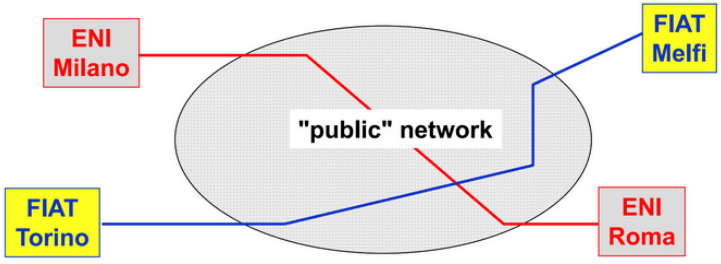
\includegraphics[width=0.5\textwidth]{/home/lorenzo/Notes/Information System Security/images/Screenshot from 2024-12-30 16-45-35.png}
    \caption{VPNs in a Public Network}
\end{figure}
A VPN can be created in three different ways:
\begin{itemize}
    \item \underline{\textbf{VPN via Private Address}}: The networks that want to be part of the VPN \textbf{must} use \textbf{Non-Public IP Addresses} that are \textbf{unreachable} from the other networks. These VPNs are considered \textbf{private} since they do not require authorization and the packets are \textbf{not} globally routable.\\   
    However, these protections can be easily defeated if somebody:
    \begin{itemize}
        \item Guesses or discovers the non-public IP addresses.
        \item Sniffs the packets during their transmission.
        \item Manages to access the communication devices.
    \end{itemize}
    \vspace{-0.2cm}
    \begin{quotebox-red}{Beware}
        This kind of VPN does not
        implement any type of protection for packets, users or the infrastructure itself \(\rightarrow \) the level of security of this solution is close to \textbf{zero}.
    \end{quotebox-red}
    \item \underline{\textbf{VPN via Tunnel}}: The routers encapsulate the whole L3 packet as the payload of another L3 packet (e.g. \textbf{IP in
    IP, IP over MPLS}, etc...). \textbf{Before} the encapsulation, the Border Routers perform \textbf{access} control to the VPN by checking an \textbf{ACL} (\textbf{Access Control List}).  
    For example, if the VPN belongs to the 10.1.0.0\textbackslash16 address range, the VPN can be accessed \textbf{only} by someone in 10.1.0.0\textbackslash16.\\    
    \\
    This solution grants VPN Providers protection against \textbf{malicious} VPN Customers, because it is impossible for Customers can change the subnet to which they belong (if they try, they do not belong anymore to the VPN).

    \begin{quotebox-red}{Beware}
        However, this protection can be defeated by anybody that \textbf{manages} a router or by Sniffing attacks \(\rightarrow \) protection works for Providers but \textbf{not} for Customers.
    \end{quotebox-red}
    \begin{quotebox-grey}{Example: VPN via IP Tunnel}
    \begin{minipage}{0.6\textwidth}
    %	\vspace{-0.5cm}
    \textbf{Net 1} and \textbf{Net 2} have got the \textbf{same color} because they belong to the \textbf{same subnet}.
    This VPN uses IP in IP Tunneling and works in the following way: 
    \begin{enumerate}
        \item \textbf{Node A} from \textbf{Net 1} sends a packet to \textbf{Node B} in \textbf{Net 2}.
        \item . The packet reaches the Border Router \textbf{R1}, which encapsulates it by adding the \textbf{IPv4 Header (Tunnel)}.
        \item The Tunneled Packet is forwarder from \textbf{R1} to \textbf{R2}.
        \item \textbf{R2} decapsulates the packet and forwards it to \textbf{Node 2}.
    \end{enumerate}
    \end{minipage} 
    \hspace{0.2cm}
    \begin{minipage}{0.4\textwidth}
        \centering
        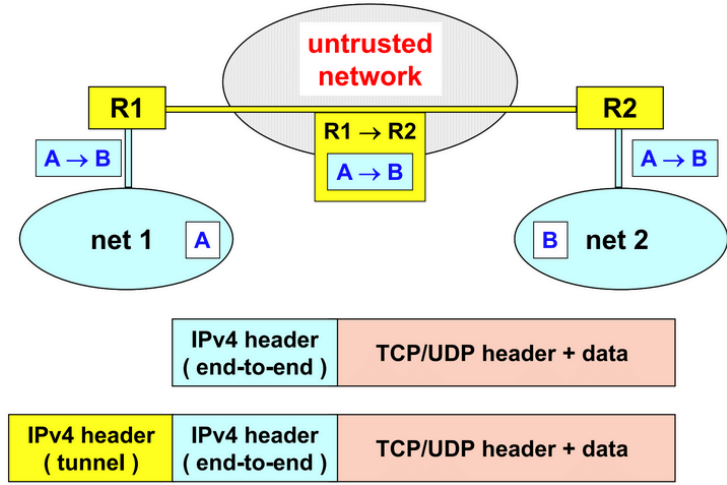
\includegraphics[width=0.9\textwidth]{/home/lorenzo/Notes/Information System Security/images/Screenshot from 2024-12-30 17-38-10.png}
    \end{minipage}
    \end{quotebox-grey}
    \item \underline{\textbf{VPN via Secure IP Tunnel}}: This type of VPN, also known as \textbf{S-VPN} (\textbf{Secure VP}), protects \textbf{also} VPN Customers. To
    do so, before encapsulation, the packets are protected with:
    \begin{itemize}
        \item \textbf{MAC}: grants \textbf{integrity} and \textbf{data authN}.
        \item \textbf{Encryption}: confidentiality.
        \item \textbf{Numbering}: to avoid Replay attacks.
    \end{itemize}
    There is \textbf{no} Digital Signature, because Asymmetric Encryption is \textbf{slow} and does \textbf{not} fit the
speed standards of modern networks. If the selected algorithms are \textbf{strong} \(\rightarrow \) only DoS attacks are possible.\\
\begin{minipage}{0.6\textwidth}
    %	\vspace{-0.5cm}
        In this picture, there are the Border Routers \textbf{R1} and \textbf{R2}, and the \textbf{TAP}s (\textbf{Tunnel Access Point}) \textbf{T1} and \textbf{T2}:
        \begin{itemize}
            \item Routers performs \textbf{encapsulation} and \textbf{decapsulatation}
            \item TAPs perform \textbf{cryptographic} and \textbf{decapsulatation}.
        \end{itemize}
    \end{minipage} 
    \hspace{0.2cm}
    \begin{minipage}{0.4\textwidth}
        \centering
        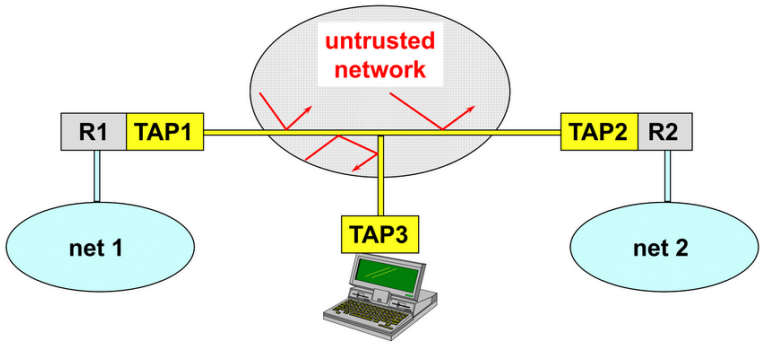
\includegraphics[width=0.9\textwidth]{/home/lorenzo/Notes/Information System Security/images/Screenshot from 2024-12-30 17-59-07.png}
    \end{minipage}
    \begin{quotebox-red}{Beware}
        If the TAP is managed by an \textbf{external} network Provider \(\rightarrow \) this is \textbf{fake security}.\\
        Security can be achieved only if there are separated devices, where:
        \begin{itemize}
            \item The TAPs are managed by the \textbf{client}.
            \item The Border Routers are be managed by the \textbf{ISP}.
        \end{itemize}
    \end{quotebox-red}
\end{itemize}
\noindent{\color{gray!50}\rule{\textwidth}{0.5pt}}
\section{IPsec}
IPSec (Internet Protocol Security) is a suite of protocols used to secure IP communications. It used to create:
\begin{itemize}
    \item \textbf{S-VPN} over \textbf{unstrusted} networks.
    \item \textbf{End-to-End secure packet flows}
\end{itemize}
IPsec defines two specific packet types:
\begin{itemize}
    \item \textbf{AH} (\textbf{Authentication Header}): provides \textbf{integrity}, \textbf{data authN} and protection against Replay attacks.
    \item \textbf{ESP} (\textbf{Encapsulating Security Payload}): provides nearly the same functions as \textbf{AH} and additionally grants \textbf{payload confidentiality}.\\    \\
    \textcolor{red}{\textbf{N.B.}} \textbf{Confidentiality} can \textbf{never} be provided for the \textbf{header}, if it is encrypted \(\rightarrow \) the intermediate systems would \textbf{not} be able to process the packets.
\end{itemize}
\noindent
Moreover, IPsec also defines \textbf{IKE} (\textbf{Internet Key Exchange}), which is a dedicated protocol for Key-Exchange.
\\ Thanks to all of these features, IPsec offers the following Security Services:
\begin{itemize}
    \item \textbf{AuthN of IP Packets}: achieved with the computation of a Keyed-Digest of the packets
    with a symmetric key. This provides:
    \begin{itemize}
        \item \textbf{Data Integrity}: the receiver can detect if the packets have been manipulated.
        \item \textbf{Sender AuthN}:  formal proof of the sender’s identity.
        \item \textbf{Partial} protection against Replay attacks \(\rightarrow \) working at L3 means that packets can be lost or duplicated.
    \end{itemize}
    \item \textbf{Confidentiality of IP Packets} \(\rightarrow \) but only for the \textbf{payload}.
    \item \textbf{Peer AuthN when Creating the SA}: when creating a \textbf{Security Association} (\textbf{SA}), a Key Agreement is needed \textbf{after} peer authN.
\end{itemize}

\subsection{SA (Security Association)}
A \textbf{SA} is an \textbf{unidirectional} logic connection between two IPsec systems. Each SA has associated a \textbf{single} and \textbf{unique} Security Service. To achieve \textbf{full protection} for a bidirectional
packet flow between two nodes, we \textbf{always} need two SAs, one A → B and one B → A.
\begin{figure}[H]
    \centering
    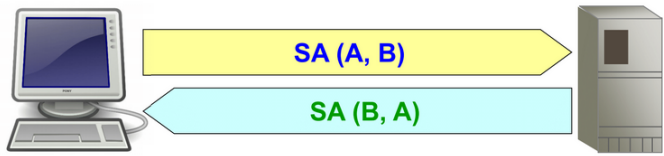
\includegraphics[width=0.5\textwidth]{/home/lorenzo/Notes/Information System Security/images/Screenshot from 2024-12-30 18-53-51.png}
\end{figure}

\subsection{Local "Database"}
SAs are managed via two \textbf{Local "Databases"}:
\begin{itemize}
    \item \textbf{SPD (Security Policy Database)}: 
\end{itemize}

